

由于软件的运行性能和处理器的结构有着非常紧密的联系,所以本节首先介绍龙芯3号系列处理器的硬件体系特点,为后续章节的优化工作做出理论基础。

\subsection{龙芯3号处理器架构介绍\cite{Loongson3A-Manual}}

龙芯3号的可伸缩互连结构如下图\ref{fig:Loongson3-System-Struct}所示。在图中,龙芯3号片内采用二维mesh互连结构,其中每个结点由8*8的交叉开关组成,每个交叉开关连接四个处理器以及分成四个体的共享二级Cache,并与东(E)南(N)西(W)北(N)四个方向的其他结点互连。因此,2*2的mesh可以连接16个处理器,4*4的mesh可以连接64个处理器。龙芯3号的互连网络采用128位支持Cache一致性的AXI(AMBA3.0)标准接口。

\begin{figure}[H] 
  \centering
  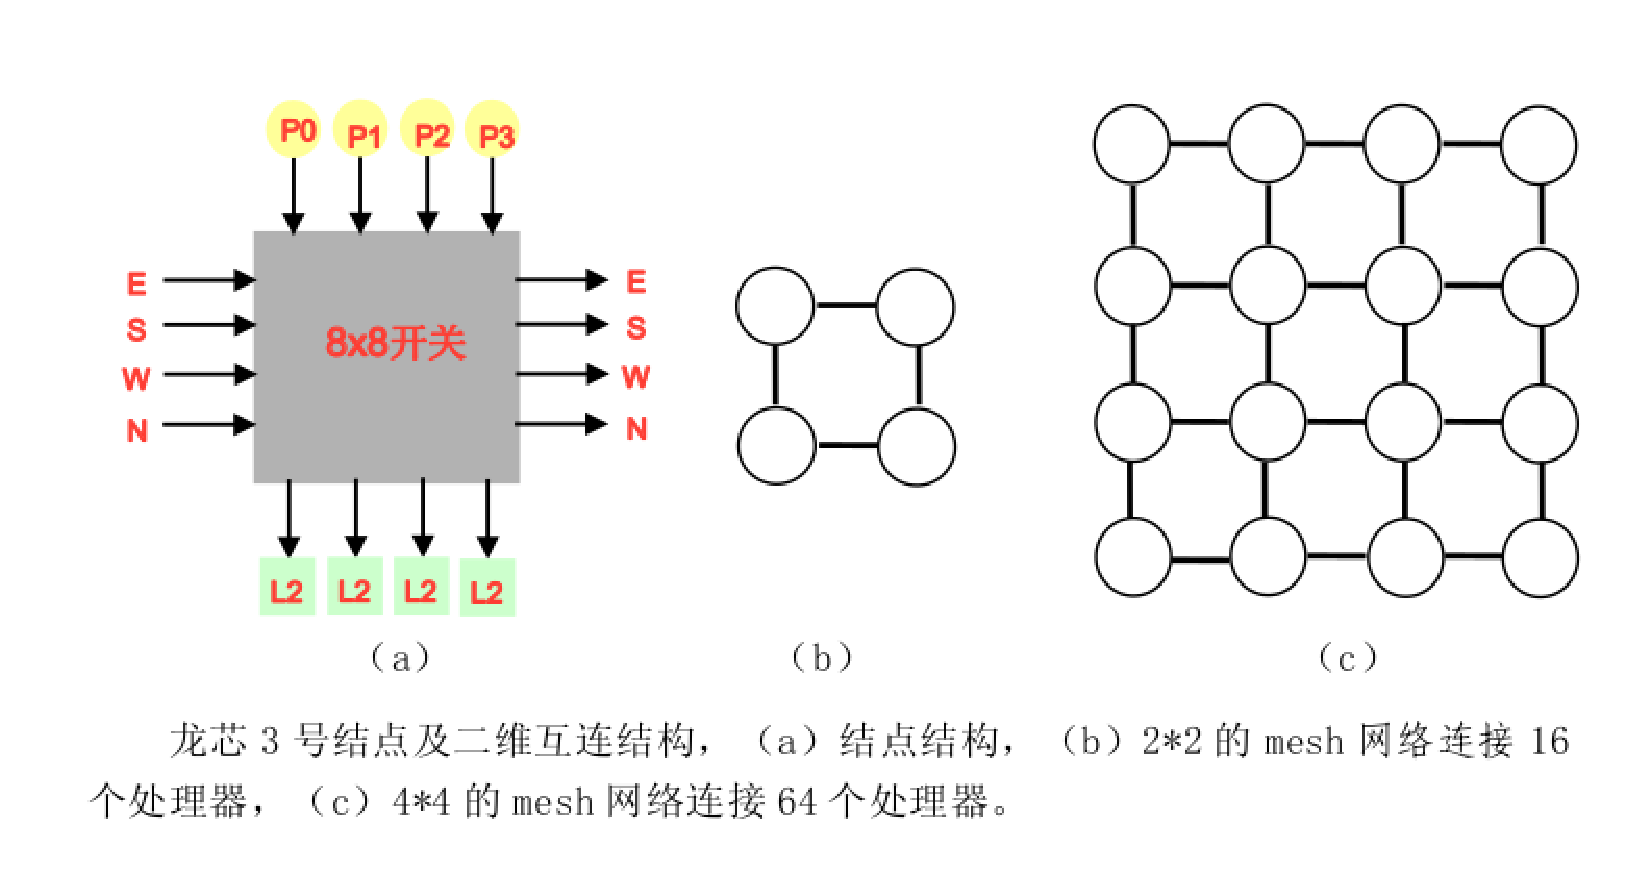
\includegraphics[width=12cm,height=7cm]{figures/chap02/Loongson3-System-Struct}
  \caption{龙芯3号系统结构}
  \label{fig:Loongson3-System-Struct}
\end{figure}

龙芯3号的片内二级Cache分布在不同的结点中,被片内的所有处理器共享。每个结点的二级Cache根据地址分成interleave的四个体,可以被并行访问。所有结点的二级Cache统一编址,每个Cache块都有一个固定的home结点,并在home结点处维护相应Cache块的目录,通过基于目录的Cache一致性协议维护一级Cache的一致性。每个结点(或多个相邻结点)对应一个DDR2内存控制器。内存地址分布和二级Cache的地址分布一致,以简化二级Cache和内存之间的通路并降低二级Cache访问失效的延迟。龙芯3号的IO控制器在边界结点上,通过边界结点空闲的交叉开关端口接入。龙芯3号的IO端口采用 HyperTransport(简称HT)协议。

龙芯3号的一般性结点结构如下图\ref{fig:Loongson3-Node-Struct}所示。每个结点有两级AXI交叉开关连接处理器、二级Cache、内存控制器以及IO控制器。其中第一级AXI交叉开关(称为X1 Switch,简称 X1)连接处理器和二级Cache,通过对AXI的扩充传递跟维护Cache一致性有关的信息。第二级交叉开关(称为X2 Switch,简称X2)连接二级Cache和内存控制器,采用标准的128位AXI协议。

\begin{figure}[H] 
  \centering
  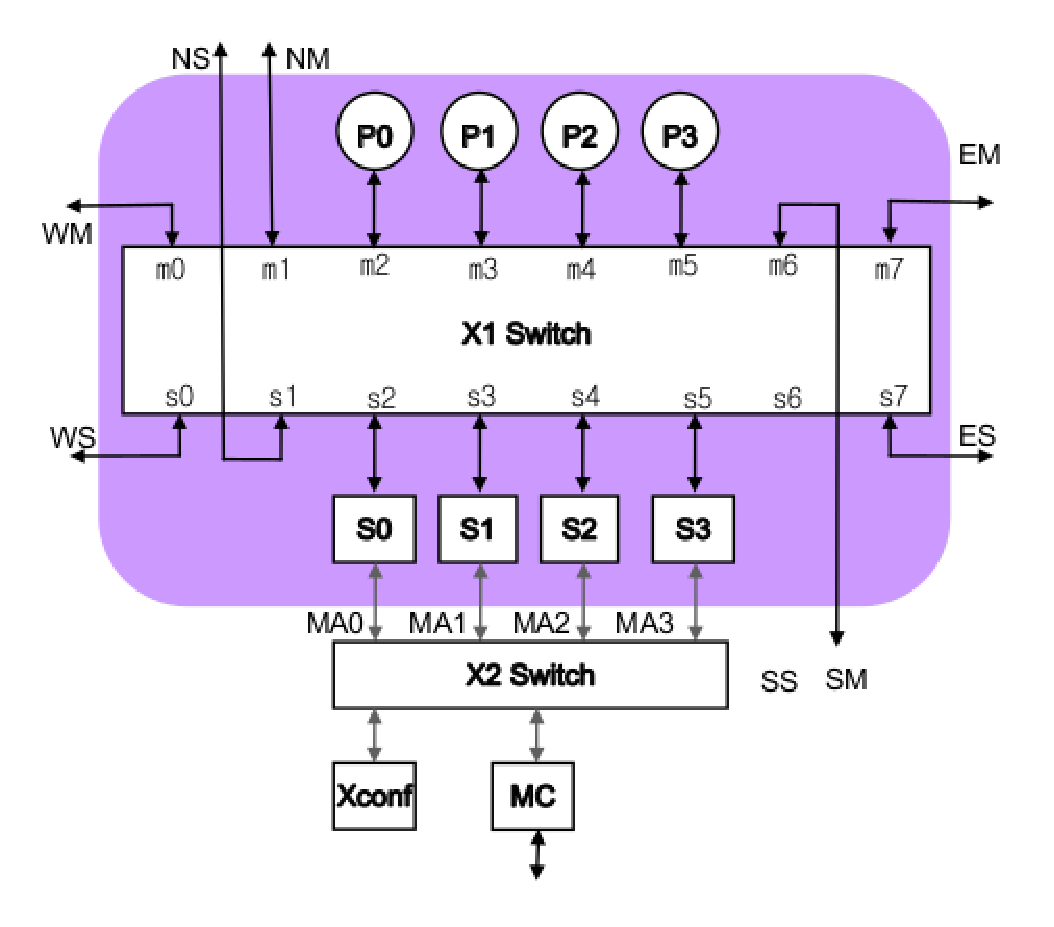
\includegraphics[width=10cm,height=7cm]{figures/chap02/Loongson3-Node-Struct}
  \caption{龙芯3号节点结构}
  \label{fig:Loongson3-Node-Struct}
\end{figure}

在每个结点中,最多8*8的X1交叉开关通过四个Master端口连接四个GS464处理器核(图中 P0、P1、P2、P3),通过四个Slave端口连接统一编址的四个 interleave二级Cache块(图中 S0、S1、S2、S3),通过四对Master/Slave端口连接东、南、西、北四个方向的其他结点或IO结点(图中 EM/ES、SM/SS、WM/WS、NM/NS)。

X2交叉开关通过四个Master端口连接四个二级Cache块,至少一个Slave端口连接一个内存控制器,至少一个Slave端口连接一个交叉开关的配置模块(Xconf)用于配置本结点的X1和X2的地址窗口等。还可以根据需要连接更多的内存控制器和IO端口等。

在龙芯3号的互连系统只是定义上层协议,会不对传输协议的实现做具体规定,因此,结点之间的互连即可以采用片上网络进行实现,也可以通过I/O控制链路实现多芯片的互连。在一个4结点16核系统为例,既可以通过4片4核芯片组成,也可以通过2片8核芯片,或基于一个单芯片4节点16核芯片组成。由于互连系统的物理实现对软件透明,上述3种配置的系统可以运行相同的操作a系统进行。

\subsection{龙芯3号平台Radeon R600系列显卡}

在龙芯3号系列处理是平台上常用到的显卡设备就是Radeon R600系列的显卡,所以这里对该显卡做简单的介绍。

\subsubsection{Radeon R600系列显卡基本介绍}

Radeon R600显卡是AMD-ATI公司开发的一个显示核心产品线,系列首张显卡HD 2900XT于2007年5月14日发表。R600系列显卡在老一代的R500系列显卡的基础上发生了很大的变化,不再包含2D加速部件,所有的加速都使用3D部件完成,使用Shader Model 4.0, 使用超标量统一着色器架构(Unified shader)。具体的新技术特征如下:

\begin{itemize}

\item{}Shader Model 4.0,统一着色架构的几何和像素支持
\item{}全速32位浮点处理
\item{}支持浮点融合,纹理过滤和抗锯齿的HDR渲染
\item{}高性能动态分支与控制流技术
\item{}采用先进的缓存系统实现几乎无限的着色指令存储
\item{}先进的纹理压缩技术
\item{}新的顶点缓存和顶点预取设计,提高顶点处理的吞吐量
\item{}实时阴影渲染的Z缓存优化

\end{itemize}

\subsubsection{Radeon R600系列显卡3D图形渲染管线}

Radeon系列显卡通过内置的3D图形流水线帮助实现图形渲染的硬件加速,这里以Radeon R600显卡为例介绍其内部的图形流水线结构。R600显卡内部图形流水线主要有以下几个阶段:

\begin{itemize}
\item{\textbf{命令处理}}: \\
命令处理器(CP)需要处理环形缓冲区的命令流。在3D渲染管线里面,命令处理器处理这些命令流的时候通常会产生一系列的写寄存器活动。驱动设置好index buffer(GTT内存)并将index buffer告知硬件,被命令触发后,顶点组装和细分器(vertex grouper and tesselator, VGT)根据index buffer的地址将索引数据DMA到SPI(shader pipe interpolator)上,同时将图元的连接信息发送给图元组装器(primitive assembly)。
\item{\textbf{顶点处理}}: \\
所有的着色处理(shader processing)都是在统一着色器块(unified shader block)中进行的,统一着色器块包含Sequencer(SQ,控制shader运行)和Shader pipe(SP)模块,每一个shader程序都能够访问一些通用寄存器,这些通用寄存器是在shader程序运行之前由SPI动态分配的,SPI会往这些寄存器中加载合适的参数,这些参数包括顶点数据的基地址。然后SPI会为SQ启动程序执行过程,shader程序需要做的第一件事情就是取顶点数据,然后针对这个顶点运行shader程序,顶点处理shader的输出被放置到着色器输出缓存(shader export,SX)中\cite{R600-ISA}。
\item{\textbf{片段处理}}: \\
顶点处理完成后,顶点数据被发送到图元组装器(PA)中进行图元组装,PA的输出被发送给扫描转换器(scan convert,SC)进行扫描转换(光栅化过程,差值计算),SC会检查深度缓存(Depth buffer,DB)确定片段的可用性,这个检查过程会进行Early Z、Re-Z和HiZ处理。光栅化出来的片段被发送给SPI,再进入到shader core里面进行最后的片段处理。片段处理器会进行取纹理、ALU计算以及内存读写操作。完成后,片段的几何信息(在屏幕坐标系中的坐标以及深度值)和颜色信息通过SX发送到DB和CB中进行最后的处理。
\item{\textbf{最后渲染}}: \\
Pixel shader的输出被放到DB和CB中进行最后的处理,这部分处理包括alpha测试、深度测试和最后的融合(blending)。
\end{itemize}

具体结构图如下图\ref{fig:R600-Pipeline}:

\begin{figure}[H] 
  \centering
  \includegraphics[width=13cm,height=15cm]{figures/chap02/R600-Pipeline}
  \caption{R600图形渲染管线}
  \label{fig:R600-Pipeline}
\end{figure}

总体上来说,输入数据大体上按照“顶点处理”、“图元组装”、“光栅化”、“片段处理”、“输出”的过程流经图形硬件。这些阶段几乎完全覆盖了前面图\ref{fig:OpenGL-Pipeline}里面的渲染过程,更加详细信息可查阅参考文献Radeon R6xx/R7xx Acceleration\cite{Radeon-Manual}。
